\documentclass[12pt]{article}
\usepackage[latin1]{inputenc}
\usepackage{graphicx,subfigure}
\topmargin -1mm
\oddsidemargin -1mm
\evensidemargin -1mm
\textwidth 155mm
\textheight 220mm
\parskip 2mm
\parindent 3mm
%\pagestyle{empty}

\begin{document}

\begin{center}

{\Large \bf The Implementation  of an Algorithm 
to calculate Thermodynamic Equilibria for 
multi-component Systems with many non-ideal Phases.

}

Bo Sundman

INSTN, CEA Saclay, France

DRAFT Version \today

\end{center}

{\bf Keywords:} Thermodynamics; Calphad; Equilibrium calculations;
Assessments; First principle data; Phase transformations; Simulations;

\abstract{Thermodynamics is a central part in materials science.
Thermodynamic models provides a unique method to combine experimental
data and results from first principle calculations in databases.
These databases are essential to provide values of many different
thermodynamic properties in software tools for simulating materials
processes and to predict their final properties.

A well established algorithm to calculate thermodynamic
equilibria for multi-component systems using different kinds of
conditions and with many non-ideal solution phases modelled in
different ways is explained in detail.  In particular how to handle
phases with variable amount of atoms and how to handle different types
of conditions and changes of the set of stable phases during
iterations.

The algorithm can also be used to calculate properties outside the
equilibrium state as required for the simulation of phase
transitions.}

\section{Introduction}

The algorithm presented here was derived and explained in slightly
different forms by Gunnar Erikssom~\cite{75Eri}, Mats
Hillert~\cite{81Hil} and in the thesis by Bo Jansson~\cite{84Jan} and
in a paper by Lukas~\cite{82Luk}.  These papers give the theoretical
background of the algorithm but they are very dense and difficult to
understand.  In this paper the algorithm and its implementation is
explained in more detail.

The implementation is done as part of the Open Calphad
initiative~\cite{11Kat} to provide a free software for thermodynamic
calculations.  This software will provide a useful link between
experimental work, first principle calculations and applications like
simulatons of phase transformations and microstructures using phase
field methods.

\section{The thermodynamic model}

Phases in a thermodynamic system can be very different, examples are
gas, liquid, amorpheous and many different crystalline forms.  In any
system the Gibbs energy, $G$, is given at equilibrium by

\begin{equation}
G = \sum_{\alpha} \aleph^{\alpha} G_m^{\alpha}(T,P,Y) \label{eq:gmsum}
\end{equation}
where $\aleph^{\alpha}$ is the number of moles of formula units of the
phase $\alpha$ and $G_m^{\alpha}$ is the Gibbs energy per mole formula
unit of $\alpha$.  Each phase can be modelled differently but its
Gibbs energy depend on the temperature, pressure and its constitution,
here denoted by $T, P$ and $Y$.

Note that this definition of the molar Gibbs energy is different from
the normal

\begin{equation}
G_m = \frac{G}{N}\label{eq:molg1}
\end{equation}
where $N$ is the total number of moles of components.  But in this
paper $G_m$ will always be used according to the definition in
eq.~\ref{eq:gmsum}, using the formula unit explained in the next
section.

At equilibrium at constant $T, P$ and overall composition will be at a
minimum in the Gibbs energy.  For other conditions like volume,
chemical potential etc we can add Lagrangian constraints to obtain
the appropriate function to minimize.  Internal constraints, that the
sum of constituent fraction on each sublattice can also be handelled
by Lagarangian multipliers.

Each phase can be described with a different model but the
explanations in this paper will mainly concern phases modelled with
the compound energy formalism (CEF)~\cite{81Sun,90Hil}.  This include
as special gases ideal gases, substitutional regular soultions,
interstitial solutions, sublattice models etc. Some additional
explanations will be given for the ionic liquid model~\cite{84Hil}.

\subsection{The formula unit of a phase}

For a phase modelled with CEF we can have sublattices and the ratio
of these are deonoted $a_s$, where $s$ is the sublattice.  For example
the $\sigma$ phase has 5 sublattices with $a_s$ equal to 2, 4, 8, 8
and 8 sites.  Sites can be whole numbers or fractions but the
recommendation is to use the smallest integer values.  Thus a Laves
phase should be modelled (A,B)$_2$(A,B)$_1$ rather than
(A,B)$_{0.666667}$(A,B)$_{0.333333}$ as the number of decimal digits
may affect the mass balance as well as the Gibbs energy.

The constituent fraction for a phase $\alpha$ are denoted
$y_i^{\alpha}$.  For a phase with sublattices there will also be a
superscript, $(s)$, $y_i^{\alpha, (s)}$ indicating the sublattice, as
the same species $i$ may be a constituent of several sublattices.
When there is no possible confusion the phase and sublattice
superscripts are often omitted and a summation over $i$ will mean for
all constituents in all sublattices.

For ease of understanding we will from now on use indices A, B etc. to
denote components or elements and indices $i, j$ etc. to denote
constituents of a phase.  In many cases a constituent of a phase is
the same as an element but it can be a molecule or ion.  The meaning
of the term component is according the the Gibbs phase rule but a
component will often be the same as an element.

The number of moles of a component A per mole formula unit of the
phase, $M^{\alpha}_{\rm A}$ is calculated as
\begin{equation}
M_{\rm A}^{\alpha} = \sum_s a_s^{\alpha} \sum_i b_{{\rm A}i} 
y_i^{\alpha, (s)} \label{eq:massfun}
\end{equation}
where $b_{{\rm A}i}$ is the stoichiometric factor of component A in
constituent $i$ and $y^{\alpha, (s)}_i$ is the fraction of constituent
$i$ in sublattice $s$ of phase $\alpha$.  As before $a_s$ is the
number of sites on sublattice $s$.  The sum of constituent fractions
on each sublattice is unity.

The total number of moles of components in a formula unit of the phase
is thus:
\begin{equation}
M^{\alpha} = \sum_{\rm A} M_{\rm A}^{\alpha}
\end{equation}
and the mole fraction is
\begin{equation}
x^{\alpha}_{\rm A} = \frac{M_{\rm A}^{\alpha}}{M^{\alpha}}
\end{equation}

The total number of moles of component A, $N_{\rm A}$, in a system
with several phases is
\begin{equation}
N_{\rm A} = \sum_{\alpha} \aleph^{\alpha} M_{\rm A}^{\alpha} \label{eq:mtot}
\end{equation}
where $\aleph^{\alpha}$ is the number of moles formula unit of the
phase $\alpha$.  The total number of moles of components, $N$, in the
system is

\begin{equation}
N = \sum_{\rm A} N_{\rm A} =
\sum_{\rm A} \sum_{\alpha} \aleph^{\alpha} M_{\rm A}^{\alpha}
\end{equation}
and the mole fraction of A in the whole system is
\begin{equation}
x_{\rm A} = \frac{N_{\rm A}}{N}
\end{equation}

We have to be careful to distinguish between $N, \aleph, M, x, y$ and
other composition related variables.

\subsection{Differentials}

The differential of $M^{\alpha}_{\rm A}$ is

\begin{equation}
dM^{\alpha}_{\rm A} = \sum_s \sum_i 
\left(\frac{\partial M_{\rm A}^{\alpha}}{\partial y_i^{\alpha, (s)}}
\right)_{y_{j\ne i}} dy_i^{\alpha, (s)} \label{eq:diffm1}
\end{equation}
where each partial derivative of $M^{\alpha}_{\rm A}$ is

\begin{equation}
\left(\frac{\partial M_{\rm A}^{\alpha}}{\partial y_i^{(s)}}
\right)_{y_{j\ne i}} = a_s^{\alpha} b_{{\rm A}i}
\end{equation}

Most of these derivatives will be zero as $M_{\rm A}$ often depends on
a single or just a few $y_i^{(s)}$.  But we can have molecules with
several atoms as constituents and also vacancies in a sublattice and
the number of moles of components per formula unt of the phase is
often not fixed.

For the ionic liquid model the situation is different as the number of
sites for cations and anions depend on the average charge on the other
sublattice.  That will be discussed in the context of that model, It
does not affect the general procedure for the minimization of the
Gibbs energy described here.

\subsection{Examples}

Understanding the meaning of formula unit is essential to the
algorithm so a few examples will be given.

\subsubsection{A gas phase with H and O}

In a gas with the molecules (H$_2$, O$_2$, H$_2$O) the moles formula
unit of the components H and O and the total number of moles in a
formula unit, $M$, are:

\begin{eqnarray*}
M_{\rm H} &=& 2y_{\rm H_2} + 2y_{\rm H_2O}\\
M_{\rm O} &=& 2y_{\rm O_2} + y_{\rm H_2O}\\
M &=& 2y_{\rm H_2} + 2y_{\rm O_2} + 3y_{\rm H_2O}
\end{eqnarray*}

The number of moles of atoms per formula unit of this gas can thus
very between 2 and 3.  The mole fractions are:

\begin{eqnarray*}
x_{\rm H} = \frac{M_{\rm H}}{M} &=& \frac{2y_{\rm H_2} + 2y_{\rm H_2O}}
{2y_{\rm H_2} + 2y_{\rm O_2} + 3y_{\rm H_2O}}\\
x_{\rm O} = \frac{M_{\rm O}}{M} &=& \frac{2y_{\rm O_2} + y_{\rm H_2O}}
{2y_{\rm H_2} + 2y_{\rm O_2} + 3y_{\rm H_2O}}
\end{eqnarray*}

\subsubsection{A crystalline phase with substitutional and interstitial
constituents}

An interstitial solution of C and N in the bcc phase in a steel with
Cr is modelled (Cr, Fe)$_1$(C, N, Va)$_3$, where Va denotes a vacancy
or vacant site.  The moles formula units of the elements are:

\begin{eqnarray*}
M_{\rm C} &=& 3y^{(2)}_{\rm C}\\
M_{\rm Cr} &=& y^{(1)}_{\rm Cr}\\
M_{\rm Fe} &=& y^{(1)}_{\rm Fe}\\
M_{\rm N} &=& 3y^{(2)}_{\rm N}\\
M &=& 1+3y^{(2)}_{\rm C}+3y^{(2)}_{\rm N}
\end{eqnarray*}

The number of moles of atoms per formula unit can thus very between 1
and 4.  He mole fractions are:

\begin{eqnarray*}
x_{\rm C} &=& \frac{3y^{(2)}_{\rm C}}{1+3y^{(2)}_{\rm C}+3y^{(2)}_{\rm N}}\\
x_{\rm Cr} &=& \frac{y^{(1)}_{\rm Cr}}{1+3y^{(2)}_{\rm C}+3y^{(2)}_{\rm N}}\\
x_{\rm Fe} &=& \frac{y^{(1)}_{\rm Fe}}{1+3y^{(2)}_{\rm C}+3y^{(2)}_{\rm N}}\\
x_{\rm N} &=& \frac{3y^{(2)}_{\rm N}}{1+3y^{(2)}_{\rm C}+3y^{(2)}_{\rm N}}\\
\end{eqnarray*}

\subsubsection{A crystalline phase with ordering}

Finally for a $\sigma$ phase in the Cr, Fe, Mo and Ni system modelled
with only 3 sublattices and with restricted solublities, (Fe,
Ni)$_{10}$(Cr, Mo)$_4$(Cr, Fe, Mo, Ni)$_{16}$, the moles formula units
are

\begin{eqnarray*}
M_{\rm Cr} &=& 4y^{(2)}_{\rm Cr} + 16y^{(3)}_{\rm Cr}\\
M_{\rm Fe} &=& 10y^{(1)}_{\rm Fe}+16y^{(3)}_{\rm Fe}\\
M_{\rm Mo} &=& 4y^{(2)}_{\rm Mo}+16y^{(3)}_{\rm Mo}\\
M_{\rm Ni} &=& 10y^{(1)}_{\rm Ni}+16y^{(3)}_{\rm Ni}\\
M &=& 30
\end{eqnarray*}

The number of moles per formula unit is constant and equal to 30.  The
mole fractions are

\begin{eqnarray*}
x_{\rm Cr} &=& \frac{4y^{(2)}_{\rm Cr} + 16y^{(3)}_{\rm Cr}}{30}\\
x_{\rm Fe} &=& \frac{10y^{(1)}_{\rm Fe}+16y^{(3)}_{\rm Fe}}{30}\\
x_{\rm Mo} &=& \frac{4y^{(2)}_{\rm Mo}+16y^{(3)}_{\rm Mo}}{30}\\
x_{\rm Ni} &=& \frac{10y^{(1)}_{\rm Ni}+16y^{(3)}_{\rm Ni}}{30}
\end{eqnarray*}

The reason for this somewhat lenghty explanation is it is very common
to make misstakes, or be uncertain using different kinds of variables
for the amount of material in a system or phase.

\subsection{End-members of models}

An important concept when modelling with CEF is the {\em end-member}
which for a crystalline phase specifies one constituent in each
sublattice of the phase.  A phase can consist o a single end-member
and for the gas phase each molecule is an end-member.  In the bcc
phase example above we have 6 end-members which can be denoted:
(Cr:C), (Cr:N), (Cr:Va), (Fe:C), (Fe:N) and (Fe:Va).  In the $\sigma$
phase example there are 16 end-members, for example (Fe:Cr:Cr),
(Fe:Cr:Fe), (Fe:Cr:Mo), (Fe:Cr:Ni) etc.  Note that in most cases
end-members represent compounds with several elements.

\section{The Gibbs energy}

The Gibbs energy, $G$ is an extensive property and can be subdivided
in may different way.  One well known formula relates the Gibbs energy
to the chemical potentials, $\mu_{\rm A}$, and the number of moles,
$N_{\rm A}$ of the components:

\begin{equation}
G = \sum_{\rm A} N_{\rm A} \mu_{\rm A} \label{eq:gsummu}
\end{equation}

The definition of the chemical potentials is

\begin{equation}
\mu_{\rm A}=\left(\frac{\partial G}{\partial N_{\rm A}}
\right)_{T,P,N_{\rm B\ne A}} \label{eq:mudef}
\end{equation}

If a phase has a fixed composition it has only a Gibbs energy and we
cannot calculate the individual chemical potentials of the components
for this phase alone.  But if we can vary the fraction of constituents
in one or more sublattices it is possible to calculate some relations
between chemical potentials as will be discussed below in the context
of eq.~\ref{eq:cmu}.

We have already introduced a different definition of the molar Gibbs
energy for each phase which is related to the formula unit of the
phase defined by structure of the phase as described above.  Using
eq.~\ref{eq:massfun} the molar Gibbs energy for a formula unit of a
phase $\alpha$ is equal to:

\begin{equation}
G_m^{\alpha} = \sum_{\rm A} M_{\rm A}^{\alpha} \mu_{\rm A}
\end{equation}

So it is important to know what kind of ``molar'' quantity we use.

\subsection{The differential of the Gibbs energy}

The differential of the Gibbs energy is

\begin{equation}
dG = -SdT+VdP+\sum_{\rm A}\mu_{\rm A}dN_{\rm A} \label{eq:dg1}
\end{equation}
and at equilibrium in a closed system $dG=0$.  If we have several
stable phases

\begin{eqnarray}
dG &=& \sum_{\alpha}(\aleph^{\alpha}dG_m^{\alpha}+G_m^{\alpha}d\aleph^{\alpha})
\end{eqnarray}
where $dG_m^{\alpha}$ for each phase can, using the molar Gibbs energy
per formula unit, be expressed as differences of the independent
variables $T, P$ and $M_{\rm A}$ or the dependent $y^{\alpha,(s)}_i$:

\begin{eqnarray}
dG_m^{\alpha} &=& -S_m^{\alpha}dT+V_m^{\alpha}dP+
\sum_{\rm A}\mu_{\rm A}dM^{\alpha}_{\rm A} \nonumber\\&=&
-S_m^{\alpha}dT+V_m^{\alpha}dP+
\sum_{\rm A}\mu_{\rm A}\sum_s \sum_i
\left(\frac{\partial M^{\alpha}_{\rm A}}{\partial y^{\alpha,(s)}_i}
\right)_{T,P,y_{j\ne i}}
dy^{\alpha,(s)}_i \label{eq:dgmfu}
\end{eqnarray}

\subsection{The partial Gibbs energy with for an end-member}

For a phase with sublattices it is not always possible to calculate
directly the chemical potentials for the components but we can always
calculate the partial Gibbs energies of the end-members, $I$, of the
model.  An end-member specifies one constituent in each sublattice:

\begin{equation}
G_I=G_m + \sum_{s}\left(\frac{\partial G_m}{\partial y^{(s)}_{i}}
\right)_{T,P,y_{j\ne i}}
- \sum_s \sum_{j} y^{(s)}_{j}\left(\frac{\partial G_m}{\partial y^{(s)}_{j}}
\right)_{T,P,y_{k\ne j}} \label{eq:mufory}
\end{equation}
where the first summation is for the constituents $i$ specified by the
end-member for each sublattice $s$.  The second double summation is
for all constituents.  For a phase with fixed composition $G_I = G_m$.

In the example for the bcc interstitial solution (Fe, Cr)$_1$(C, N,
Va)$_3$ above it is not possible to express directly the partial Gibbs
energy for C in the model.  However, we have the end-members (Fe:Va)
and (Fe:C) and we can calculate these two partials from the model:

\begin{eqnarray}
G_{\rm Fe:Va}&=&G_m + \left(\frac{\partial G_m}{\partial y^{(1)}_{\rm Fe}}
\right)_{T,P,y_{j\ne {\rm Fe}}} +
\left(\frac{\partial G_m}{\partial y^{(2)}_{\rm Va}}
\right)_{T,P,y_{j\ne {\rm Va}}}
- \sum_s \sum_{j} y^{(s)}_{j}\left(\frac{\partial G_m}{\partial y^{(s)}_{j}}
\right)_{T,P,y_{k\ne j}} \nonumber\\&&\\
G_{\rm Fe:C}&=&G_m + \left(\frac{\partial G_m}{\partial y^{(1)}_{\rm Fe}}
\right)_{T,P,y_{j\ne {\rm Fe}}} +
\left(\frac{\partial G_m}{\partial y^{(2)}_{\rm C}}
\right)_{T,P,y_{j\ne {\rm C}}}
- \sum_s \sum_{j} y^{(s)}_{j}\left(\frac{\partial G_m}{\partial y^{(s)}_{j}}
\right)_{T,P,y_{k\ne j}} \nonumber\\&&
\end{eqnarray}

At equilibrium the partial Gibbs energies of the end-members are
related to the chemical potentials of the components as

\begin{eqnarray*}
G_{\rm FeVa_3} = G_{\rm Fe:Va} = G_{\rm Fe} &=& \mu_{\rm Fe}\\
G_{\rm FeC_3} = G_{\rm Fe:C} = G_{\rm Fe} + 3G_{\rm C} &=&
\mu_{\rm Fe} + 3\mu_{\rm C}
\end{eqnarray*}
as the chemical potential of Va, $\mu_{\rm Va}=0$ at equilibrium.  We
can rearrange to obtain the chemical potential of C:

\begin{eqnarray}
\mu_{\rm C} = G_{\rm C} = \frac{1}{3}(G_{\rm Fe:C}-G_{\rm Fe:Va}) &=&
\frac{1}{3}\left[\left(\frac{\partial G_m}{\partial y^{(2)}_{\rm C}}
\right)_{T,P,y_{\rm Va}} -
\left(\frac{\partial G_m}{\partial y^{(2)}_{\rm Va}}
\right)_{T,P,y_{\rm C}}\right] \label{eq:cmu}
\end{eqnarray}

As can be seen by the last part of eq.~\ref{eq:cmu} it is independent
of the constituent in the first sublattice so it does not matter if we
had chosen the end-members (Cr:C) and (Cr:Va).  At equilibrium the
difference will be the same.  And even of there is no Cr so Fe is
alone on its sublattice we can obtain the chemical potentials of both
Fe and C because the fraction of C can vary.

It is not possible to combine end-members in all possible CEF models
to extract the chemical potentials of the elements, in the model for
for the $\sigma$ phase above we cannot obtain the individual chemical
potentials of the elements from the model.  But the method described
below to calculate the equilibrium can be applied also for such
phases.

%\begin{eqnarray*}
%\end{eqnarray*}

\subsection{The Gibbs-Duhem relation}

In eq.~\ref{eq:dg1} there is no differential of the chemical
potentials because the Gibbs-Duhem relation for each phase is:

\begin{equation}
\sum_{\rm A}d\mu_{\rm A} M^{\alpha}_{\rm A}+S_m^{\alpha}dT+V_m^{\alpha}dP =0
\end{equation}
which must be valid at equilibrium.  

\section{Minimization with constraints}

To minimize a function with constraints we apply a Lagarangian
equation where each equality constraints has a multiplier.  When the
constraint is obeyed the minimim of the Lagrangian is the same as the
origibal function.  The multipliers can be used to find the method to
vary the variables to fulfill the constraints.

\subsection{The constraints}

The variables in the Gibbs energy expression have several constraints.
The first is that the sum of the site fractions on each sublattice is
unity:

\begin{equation}
g^{\alpha}_s = 1 - \sum_i y^{\alpha,(s)}_i = 0
\end{equation}

For phases with ions the net charge must be zero and an external
charge balance constraint must be added:

\begin{equation}
Q^{\alpha} = \sum_s a_s \sum_i \nu_i y^{\alpha,(s)}_i = 0 \label{eq:qsum}
\end{equation}

\noindent
where $\nu_i$ is the charge on constituent $i$.

The total Gibbs energy for a system, $G$, is given by
eq.~\ref{eq:gmsum}.  The number of formula units of a phase $\alpha$,
$\aleph^{\alpha}$, must be equal to or larger than zero for a stable
phase.  If it becomes negative during iterations it will be removed
from the stable set of phases.

For a closed system we have the constraint on the amount of components

\begin{equation}
f_{\rm A}={\tilde N}_{\rm A}-N_{\rm A}={\tilde N}_{\rm
A}-\sum_{\alpha}\aleph^{\alpha}M^{\alpha}_{\rm A}=0
\end{equation}

\noindent
where ${\tilde N}_{\rm A}$ is the prescribed amount of component A.
For a phase modelled (A,B)$_{0.75}$(A,B)$_{0.25}$ the value of
$\aleph^{\alpha}$ is 4 times larger compared to the case that the
phase had been modelled (A,B)$_3$(A,B)$_1$.  Both models are allowed
and the thermodynamic parameters in the second case must be 4 times
larger than those in the first.

\subsection{The Lagrangian}

To minimize the Gibbs energy of a system with constraints we can use a
Lagrangian as

\begin{equation}
L = G + \sum_{\rm A} f_{\rm A} \mu_{\rm A} + 
\sum_{\alpha} \eta_s^{\alpha} g_{s}^{\alpha} +
\sum_{\alpha} \lambda^{\alpha} Q^{\alpha} + 
\sum_{\psi} \gamma^{\psi} \aleph^{\psi}
\end{equation}

\noindent
where $\mu_{\rm A}, \eta_{s}^{\alpha}, \lambda^{\alpha}$ are
multipliers for all phases and $\gamma^{\psi}$ are multipliers for all
phases $\psi$ that are unstable with $\aleph^{\psi}=0$.  The
important property of this Lagrantian is that it will have the same
extremum points as the Gibbs energy $G$ when the constraints are
fullfilled.  From now on it will rarely be indicated which variables
are kept constant at the partial derivatives, the reader is expected
to understand this from the text.

For the partial derivative of $L$ with respect to the amount of a
stable phase $\alpha$ we get:

\begin{equation}
\frac{\partial L}{\partial \aleph^{\alpha}} = G^{\alpha}_m - 
\sum_{\rm A} f_{\rm A} M^{\alpha}_{\rm A} = 0
\end{equation}
and from this equation we can understand that the Lagrangian
multiplier $f_{\rm A} = \mu_{\rm A}$, i.e. the chemical potential of
component A.  For a rigorous proof see~\cite{81Hil}.

For an unstable phase $\psi$ which is not included in the stable
phase set:

\begin{equation}
\frac{\partial L}{\partial \aleph^{\psi}} = G^{\psi}_m - 
\sum_i \mu_i M^{\psi_i} + \gamma^{\psi} = 0 \label{eq:dgm1}
\end{equation}

This means that the driving force, $\gamma^{\psi}$, for an unstable
phase will be calculated as part of the minimization.  An unstable
phase may become stable during the iterations for the equilibrium and
that is indicated by $\gamma^{\psi}$ becomming positive.  If
$\aleph^{\alpha}$ for a stable phase $\alpha$ becomes negative it
means this phase has become unstable and should be removed from the
stable set.  In both cases we must change the set of stable phases as
will be discussed below.

The partial derivative of $L$ with respect to a constituent fraction
$y^{\alpha,(s)}_i$, keeping all other variables constant, we get:

\begin{equation}
\frac{\partial L}{\partial y^{\alpha,(s)}_i} =
\aleph^{\alpha}\frac{\partial G_m^{\alpha}}{\partial y^{\alpha,(s)}_i} -
\aleph^{\alpha}\sum_{\rm A} \mu_{\rm A} 
\frac{\partial M^{\alpha}_{\rm A}}{\partial y^{\alpha,(s)}_i}-
\eta^{\alpha}_s+
\lambda^{\alpha}\frac{\partial Q^{\alpha}}{\partial y^{\alpha,(s)}_i}
 = 0\label{eq:dldy}
\end{equation}

We would like to use this equation in an iterative procedure to find
the equilibrium and to obtain a linear correction of the difference
between the current value of the constituent fractions and those of
the equilibrium we expand the partial derivative of $\frac{\partial
G_m^{\alpha}}{\partial y^{\alpha,(s)}_i}$ in a Taylor series of its
idependent variables $dT, dP$ and $dy_j^{\alpha,(t)}$:

\begin{eqnarray}
\frac{\partial G_m^{\alpha}}{\partial y^{\alpha,(s)}_i} &=&
\left(\frac{\partial G^{\alpha}_m}{\partial y^{\alpha,(s)}_i}\right)
+\left(\frac{\partial^2 G_m^{\alpha}}{\partial y^{\alpha,(s)}_i\partial T}\right) dT
+\left(\frac{\partial^2 G_m^{\alpha}}{\partial y^{\alpha,(s)}_i\partial P}\right) dP
+\sum_t\sum_{j}\left(\frac{\partial^2  G^{\alpha}_m}
{\partial y^{\alpha,(s)}_i y^{\alpha,(t)}_j}\right)dy^{\alpha,(t)}_j
\nonumber\\\label{eq:taylor3}
\end{eqnarray}
where the terms on the right hand side are calculated for the current $T,
P$ and $Y_i$ and the term on the left hand side is the linearly
``extrapolated'' value.  The last term on the right hand side is a
summation over all constituents $j$ on all sublattices $t$.  In the
rest of this paper it will often be written as just a summustion over
$j$.

Inserting this in eq.~\ref{eq:dldy} and changing to finite differences
we get a system of linear equations depending on the corrections in
$\Delta T, \Delta P$ and $\Delta y^{\alpha,(s)}_i$:

\begin{eqnarray}
\sum_t \sum_{j}\left(\frac{\partial^2  G^{\alpha}_m}
{\partial y^{\alpha,(s)}_i y^{\alpha,(t)}_j}\right)\Delta y^{\alpha,(t)}_j
+\frac{\eta^{\alpha}_s}{\aleph^{\alpha}} &=&\nonumber\\
\sum_{\rm A} \mu_{\rm A} \left(\frac{\partial M^{\alpha}_{\rm A}}
{\partial y^{\alpha,(s)}_i}\right) -
\left(\frac{\partial G^{\alpha}_m}{\partial y^{\alpha,(s)}_i}\right) &-&
\left(\frac{\partial^2 G_m^{\alpha}}{\partial y^{\alpha,(s)}_i\partial T}\right) \Delta T
-\left(\frac{\partial^2 G_m^{\alpha}}{\partial y^{\alpha,(s)}_i\partial P}\right)\Delta P
\nonumber\\&&\label{eq:phasemat2}
\end{eqnarray}

We are intersted to solve this for the fraction corrections $\Delta
y_i$ and can rearrange this in matrix notation, omitting the
superscripts:

\refstepcounter{equation}\label{eq:phasematrix1}

\[ 
\left(
\begin{tabular}{ccccc}
$\frac{\partial^2 G_m}{\partial y^2_1}$ &
$\frac{\partial^2 G_m}{\partial y_1\partial y_2}$ & $\cdots$ & 1 & $\cdots$ \\
\\
$\frac{\partial^2 G_m}{\partial y_1\partial y_2}$ & 
$\frac{\partial^2 G_m}{\partial y^2_2}$ & $\cdots$ & 1 & $\cdots$ \\
\\
$\vdots$ \\
\\
1 & 1 & $\cdots$ & 0 & $\cdots$ \\
\\
$\vdots$\\
\end{tabular}
\right)
\left(
\begin{tabular}{c}
$\Delta y_1$\\
\\
$\Delta y_2$\\
\\
$\vdots$\\
\\
$\frac{\eta_1}{\aleph}$\\
\\
$\vdots$\\
\end{tabular}
\right) 
=
\left(
\begin{tabular}{c}
$\sum_{\rm A} \mu_{\rm A}
\frac{\partial M_{\rm A}}{\partial y_1}
-\frac{\partial G_m}{\partial y_1}
-\frac{\partial^2 G_m}{\partial y_1\partial T}\Delta T
-\frac{\partial^2 G_m}{\partial y_1\partial P}\Delta P$\\
\\
$\sum_{\rm A} \mu_{\rm A}
\frac{\partial M_{\rm A}}{\partial y_2}
-\frac{\partial G_m}{\partial y_2}+
\frac{\partial S_m}{\partial y_2}\Delta T-
\frac{\partial V_m}{\partial y_2}\Delta P$\\
\\
$\vdots$\\
\\
0\\
\\
$\vdots$\\
\end{tabular}
\right)
\\ 
\\ (\ref{eq:phasematrix1})
\]

The matrix on the left hand side is symmetric and the columns and rows
with 1 represent the constraint that sum of constituent fractions on
each sublattice is unity.  Inverting this {\em phase matrix} we can
express the corrections of the constuent fractions of each phase in
the global potentials $\mu_{\rm A}, \Delta T$ and $\Delta P$.  The use
of the inverted phase matrix will be explained in more detail for
several specific cases below.

\section{Calculating the equilibrium}

The solution must be calculated by an iterative process and each
iteration is divided into two steps.  To simplify the explanations a
substitutional binary system (A,B) is used in many cases.  As
discussed below there is an initial step 0 to find a good start set of
stable phases and their constitutions.

\subsection{Step 0, Obtaining start values by grid minimizer}

An iterative procedure for calculating the equilibria can only find a
local equilibrium which depend on the intitial constitution of the
phases and it is thus necessary to provide a reasonable estimate of
the stable phases and constitution of all phases for the first step.
The method to do is here is copied from the method to solve the
equilibrium for the case when all phases have a fixed composition.
Such an equilibrium is easily found by a combination of simplex and
steepest decent methods.  In such a calculation we will always find
as many stable phases as we have components.

\begin{figure}[!h]
\begin{center}
\subfigure[]{
\includegraphics[width=30mm]{figs/g1.ps}}
\subfigure[]{
\includegraphics[width=30mm]{figs/g2.ps}}
\subfigure[]{
\includegraphics[width=30mm]{figs/g3.ps}}
\subfigure[]{
\includegraphics[width=30mm]{figs/g4.ps}}\\
\subfigure[]{
\includegraphics[width=30mm]{figs/g5.ps}}
\subfigure[]{
\includegraphics[width=30mm]{figs/g6.ps}}
\subfigure[]{
\includegraphics[width=30mm]{figs/g7.ps}}
\subfigure[]{
\includegraphics[width=30mm]{figs/g4.ps}}
\end{center}
\caption{A case where start values matters.  In (a) the Gibbs energy
curves for two phases with miscibility gaps in a binary system are
shown.  If we have the initial constitutions marked in (b) the present
algorithm will find the local equilibrium shown in (c) which is not
the global minimum, the global minimum is shown in (d).  In order to
find good start values of the phases we can replace the Gibbs energy
curves with calculated gridpoints as shown in (e) and then minimize
these Gibbs energy of these gridpoints, exah treated as a separate
phase with fixed composition as shown in (f).  The grid minimizer will
find the two gridpoints joined by a line in (g) as a minimum and using
these compositions as startpoint for the calculation will give the
correct global minimum using the present algorithm as in
(h).}\label{fg:grid1}
\end{figure}

The same technique can be adopted to eystems with solution phases by
calculating a number of gridpoints in each phase and then treat each
of these as a separate phse.  The number of gridpoint does not have to
be very large even in multicomponent systems, normally 2000 points in
each phase is sufficient even with more than 10 components.  After
finding the gridpoints represpenting the equilibrium we must check if
some of them are in the same solution phase and check if they can be
merged to a single point.  That is not always the case if there are
miscibility gaps in the solution phase.  In Fig.~\ref{fg:grid1} a
case with two phases with miscibility gaps are shown.

The grid minimizer can also be used after an iterative equilibrium
calculation to check if there are gridpoints below the calculated
equilibrium surface.  Such a technique is useful if the conditions
does not allow an initial search for a grid minimum, for example if
the value of $T$ is not a condition.

If an equilibrium has already been calculated with almost the same
conditions, like while performing a STEP calculation for a property
diagram or MAP calculation for a phase diagram, it is not necessary to
perform a grid minimization again but we can use the already
calculated constitutions of the phases as start values.  But it is
important that now and again check if the current equilibrium is the
global one as we may step into a miscibility gaps that is not stable
initially and which is not detected by an iterative method.

It is also possible that the set of conditions does not allow a global
gridminimization, for example if $T$ is not known.  In such cases we
can start from a default initial constitution of the phases and after
the equilibrium has been calculated, and the value of $T$ is known and
we can make a grid minimization to find if the calculated equilibrium
is indeed the globally stable.  If not the set of phases found by the
grid minimizer are used to calculate the equilibrium again.

\subsection{Step 1, the phase matrix}

The derivation will first be given for a binary system, then it will
be generallized.

\subsubsection{The phase matrix for a binary system}

For a substitutional binary phase (A,B) we can write the system of
equations from eq.~\ref{eq:phasemat2} as

\refstepcounter{equation}\label{eq:phasematrix2}

\[ 
\left(
\begin{tabular}{ccc}
$\frac{\partial^2 G_m^{\alpha}}{\partial y^2_{\rm A}}$ &
$\frac{\partial^2 G_m^{\alpha}}{\partial y_{\rm A}\partial y_{\rm B}}$ & 1 \\
\\
$\frac{\partial^2 G_m^{\alpha}}{\partial y_{\rm A}\partial y_{\rm B}}$ & 
$\frac{\partial^2 G_m^{\alpha}}{\partial y^2_{\rm B}}$ & 1\\
\\
1 & 1 & 0\\
\end{tabular}
\right)
\left(
\begin{tabular}{c}
$\Delta y_{\rm A}$\\
$\Delta y_{\rm B}$\\
$\lambda$
\end{tabular}
\right)
=
\left(
\begin{tabular}{c}
$-\frac{\partial G_m}{\partial y_{\rm A}}
-\frac{\partial^2 G_m}{\partial y_{\rm A}\partial T}\Delta T
-\frac{\partial^2 G_m}{\partial y_{\rm A}\partial P}\Delta P
+\mu_{\rm A}\frac{\partial M_{\rm A}}{\partial y_{\rm A}}
+\mu_{\rm B}\frac{\partial M_{\rm B}}{\partial y_{\rm A}}$\\
\\
$-\frac{\partial G_m}{\partial y_{\rm B}}
-\frac{\partial^2 G_m}{\partial y_{\rm B}\partial T}\Delta T
-\frac{\partial^2 G_m}{\partial y_{\rm B}\partial P}\Delta P
+\mu_{\rm A}\frac{\partial M_{\rm A}}{\partial y_{\rm B}}
+\mu_{\rm B}\frac{\partial M_{\rm B}}{\partial y_{\rm B}}$\\
\\
0
\end{tabular}
\right)\label{eq:binpm}
\\ (\ref{eq:phasematrix2})
\]


On the left hand side we have the phase matrix for the binary (A,B)
system, including the constraint that the sum of constituent fractions
is unity:

\[ \left(
\begin{tabular}{ccc}
$\frac{\partial^2 G_m^{\alpha}}{\partial y^2_{\rm A}}$ &
$\frac{\partial^2 G_m^{\alpha}}{\partial y_{\rm A}\partial y_{\rm B}}$ & 1 \\
\\
$\frac{\partial^2 G_m^{\alpha}}{\partial y_{\rm A}\partial y_{\rm B}}$ & 
$\frac{\partial^2 G_m^{\alpha}}{\partial y^2_{\rm B}}$ & 1\\
\\
1 & 1 & 0\\
\end{tabular}
\right) \]

Before calculating the second derivatives in this matrix the
constituent fractions should be checked that they are larger than a
minimal (positive) value and normalized so the sum is unity.  We
cannot solve eq.~\ref{eq:binpm} now as $\Delta T, \Delta P$ and
$\mu_{\rm A}$ are not known but we can invert the phase matrix and as
we will use that several times below we write the inverted matrix as:

\[ \left(
\begin{tabular}{ccc}
$e_{11}$ & $e_{12}$ & $e_{13}$ \\
$e_{21}$ & $e_{22}$ & $e_{23}$ \\
$e_{31}$ & $e_{32}$ & $e_{33}$ \\
\end{tabular}
\right) \]

Only a part of this matrix is important because we are not interested
in the $\lambda$ multiplier.  We can write the solution for $\Delta
y_{\rm A}$ and $\Delta y_{\rm A}$ as:

\refstepcounter{equation}\label{eq:phasemmatrix0}

\[ \left(
\begin{tabular}{c}
$\Delta y_{\rm A}$\\
$\Delta y_{\rm B}$\\
\end{tabular}
\right) 
=
\left(
\begin{tabular}{cc}
$e_{11}$ & $e_{12}$  \\
$e_{21}$ & $e_{22}$  \\
\end{tabular}
\right) 
\left(
\begin{tabular}{c}
$-\frac{\partial G_m}{\partial y_{\rm A}}
-\frac{\partial^2 G_m}{\partial y_{\rm A}\partial T}\Delta T
-\frac{\partial^2 G_m}{\partial y_{\rm A}\partial P}\Delta P+
\mu_{\rm A}\frac{\partial M_{\rm A}}{\partial y_{\rm A}}+
\mu_{\rm B}\frac{\partial M_{\rm B}}{\partial y_{\rm A}}$\\
$-\frac{\partial G_m}{\partial y_{\rm B}}
-\frac{\partial^2 G_m}{\partial y_{\rm B}\partial T}\Delta T
-\frac{\partial^2 G_m}{\partial y_{\rm B}\partial P}\Delta P+
\mu_{\rm A}\frac{\partial M_{\rm A}}{\partial y_{\rm B}}+
\mu_{\rm B}\frac{\partial M_{\rm B}}{\partial y_{\rm B}}$\\
\end{tabular}
\right) 
\\
(\ref{eq:phasemmatrix0})
\]

This gives a very important relation between the finite difference of
a site fraction expressed as a function of several derivatives of the
Gibbs energy and the ``multipliers'' $\mu_{\rm A}$, which are
identical to the chemical potentials.  This relation be used several
times below.  Writing the equation explicitly for constituent $1$,
using $e_{ij}$ for the inverted phase matrix, gives:

\begin{eqnarray}
\Delta y_{1} &=& e_{11}\left(-\frac{\partial G_m}{\partial y_{1}}
-\frac{\partial^2 G_m}{\partial y_{1}\partial T}\Delta T 
-\frac{\partial^2 G_m}{\partial y_{1}\partial P}\Delta P +
\mu_{\rm A}\frac{\partial M_{\rm A}}{\partial y_{1}} +
\mu_{\rm B}\frac{\partial M_{\rm B}}{\partial y_{1}}\right)+\nonumber\\&&
e_{12}\left(-\frac{\partial G_m}{\partial y_{2}} 
-\frac{\partial^2 G_m}{\partial y_{2}\partial T}\Delta T 
-\frac{\partial^2 G_m}{\partial y_{2}\partial P}\Delta P +
\mu_{\rm A}\frac{\partial M_{\rm A}}{\partial y_{2}} +
\mu_{\rm B}\frac{\partial M_{\rm B}}{\partial y_{2}}\right)\label{eq:deltay1}
\end{eqnarray}

\subsubsection{The general equation for the correction of 
constituent fractions}

Generallizing eq.~\ref{eq:deltay1} to any number of constituents gives
for each constituent $i$ on sublattice $s$:

\begin{eqnarray}
\Delta y^{(s)}_i&=& c_{iG} + c_{iT}\Delta T + c_{iP}\Delta P +
\sum_{\rm A} c_{i{\rm A}}~\mu_{\rm A} \label{eq:deltay}
\end{eqnarray}
where the coefficients in this equation can be calculated as:

\begin{eqnarray}
c_{iG} &=& -\sum_t\sum_j e_{ij}
\frac{\partial G_m}{\partial y^{(t)}_j}\nonumber\\
c_{iT} &=& -\sum_t\sum_j e_{ij}
\frac{\partial^2 G_m}{\partial T \partial y^{(t)}_j}\nonumber\\
c_{iP} &=& -\sum_t\sum_j e_{ij}
\frac{\partial^2 G_m}{\partial P \partial y^{(t)}_j}\label{eq:defciz}\\
c_{i{\rm A}} &=& \sum_t\sum_j e_{ij} 
\frac{\partial M_{\rm A}}{\partial y^{(t)}_j}\nonumber
\end{eqnarray}
where $i$ is the constituent in sublattice $s$ and the summation over
$j$ is for all constituents all sublattices $t$.  A is a component.
These coefficients will be used in step 2 below and also later.

As already mentioned we cannot calculate $\Delta y_i^{(s)}$ at present
because the values of $\Delta T, \Delta P$ and $\mu_{\rm A}$ are not
known.


\subsection{Charge balance}

If some constituents have a net charge we must add the differential
of eq.~\ref{eq:qsum} to ensure that the phase is electrcally neutral.

\begin{eqnarray}
Q^{\alpha} &=& \sum_s a_s \sum_i \nu_i y^{\alpha,(s)}_i = 0\\
\Delta Q^{\alpha} &=& \sum_s a_s \sum_i \frac{\partial Q}
{\partial y^{\alpha,(s)}_i} \Delta y^{\alpha,(s)}_i
\end{eqnarray}
where

\begin{eqnarray}
\frac{\partial Q^{\alpha}}{\partial y^{\alpha,(s)}_i} &=& a_s \nu_i
\end{eqnarray}

This equation is part of the phase matrix, it should be the last row
and column, call it $q$.  After inverting the phase matrix the
correction of the constituent fractions, eq.~\ref{eq:deltay}, will
have an additional term

\begin{eqnarray}
\Delta y^{\alpha,(s)}_i &=& c_{iG} + c_{iT}\Delta T + c_{iP}\Delta P +
\sum_{\rm A} c_{i{\rm A}}~\mu_{\rm A}- e_{iQ} Q^{\alpha} \label{eq:dydq}
\end{eqnarray}
where $e_{iQ}$ are the last column in the inverted phase matrix and
$Q^{\alpha}$ is the current charge of the phase.

As mentioned above a more complicated case is the ionic liquid model
where the the cation and anion site ratios depend on the charge of
the opposite site.  In such a case there is no extra equation for the
charge balanace but we cannot use that the derivatives $\frac{\partial
M_{\rm A}}{\partial y_i^{(s)}}$ are constant.

\subsection{Step 2, the external conditions}

After calculating the inverted phase matrices for all phases and
saving them we must calculate new values of the intensive variables
($\Delta T, \Delta P$ and $\mu_i$) by making use of the external
conditions.  The most common set of external conditions are fixed $T,
P$ and amount of the components, i.e. mass balance conditions.  Here
we now describe how to formulate the equations that can determine
these. 

For each stable phase $\alpha$ we will have an equation:

\begin{equation}
G_m^{\alpha} = \sum_{\rm A} M^{\alpha}_{\rm A}\mu_{\rm A} \label{eq:gmalpha}
\end{equation}

For equilibrium calculations with variable $T$ and $P$ we must take
into account any changes in these:

\begin{equation}
G_m^{\alpha} = \sum_{\rm A} M^{\alpha}_{\rm A}\mu_{\rm A} 
-\frac{\partial G_m}{\partial T}\Delta T
-\frac{\partial G_m}{\partial P}\Delta P\label{eq:gmalpha2}
\end{equation}

The other equations depend on the conditions and the number of stable
phases.

\subsubsection{Condition on the amount of the components}

The amount of each element summed over all phases is:

\begin{equation}
N_{\rm A}- {\tilde N_{\rm A}} = \sum_{\alpha}
\aleph^{\alpha}M^{\alpha}_{\rm A} - {\tilde N_{\rm A}}=0\label{eq:totaln}
\end{equation}
where ${\tilde N_{\rm A}}$ is the prescribed amount of moles of
component A.  The differential of $N$ is

\begin{eqnarray}
\Delta N_{\rm A}&=&\sum_{\alpha} \aleph^{\alpha}\Delta M^{\alpha}_{\rm A}+
\sum_{\alpha} \Delta \aleph^{\alpha}M^{\alpha}_{\rm A} = 0\label{eq:diffN1}
\end{eqnarray}

From eq.~\ref{eq:diffm1} we have:

\begin{eqnarray}
\Delta M_{\rm A}^{\alpha} &=& 
\sum_i \frac{\partial M_{\rm A}^{\alpha}}{\partial y_i^{\alpha}} 
\Delta y_i^{\alpha}
\end{eqnarray}
where the summation over $i$ is for all constituents so we have
omitted the sublattice index.  We can approximate the differentials
with finite differences and for $\Delta y_i^{\alpha}$ we now use
eq.~\ref{eq:deltay} and can write, omitting the phase superscripts and
using the coefficients $c_{iZ}$ defined in eq.~\ref{eq:defciz}:

\begin{eqnarray}
\Delta M_{\rm A} = 
\sum_{\rm B} \mu_{\rm B} 
\sum_i \frac{\partial M_{\rm A}}{\partial y_i} c_{i{\rm B}} -
\sum_i \frac{\partial M_{\rm A}}{\partial y_i} c_{iG}-
\Delta T\sum_i \frac{\partial M_{\rm A}}{\partial y_i} c_{iT}-
\Delta P\sum_i \frac{\partial M_{\rm A}}{\partial y_i} c_{iP}
\label{eq:diffm2}
\end{eqnarray}
where the sum over B is for all components.  For fixed $T$ and $P$
this becomes:

\begin{eqnarray}
\Delta M_{\rm A} = 
\sum_{\rm B} \mu_{\rm B} 
\sum_i \frac{\partial M_{\rm A}}{\partial y_i} c_{i{\rm B}} -
\sum_i \frac{\partial M_{\rm A}}{\partial y_i} c_{iG}
\label{eq:diffmnoTP}
\end{eqnarray}

\subsubsection{Example: a binary system with a single stable phasse}

If apply this to a binary A-B system with just one stable phase the
sum of the fractions of A and B in this must fullfill the mass balance
for each component we can insert this in eq.~\ref{eq:diffN1}:

\begin{eqnarray}
\Delta N_{\rm A}&=&\aleph \left(
\sum_{\rm B} \mu_{\rm B} 
\sum_i \frac{\partial M_{\rm A}}{\partial y_i} c_{i{\rm B}} -
\sum_i \frac{\partial M_{\rm A}}{\partial y_i} c_{iG}\right) +
\Delta \aleph M_{\rm A} = 0
\end{eqnarray}
and rearranging the terms we have for each element:

\begin{eqnarray}
\aleph \sum_i \frac{\partial M_{\rm A}}{\partial y_i} c_{iG} &=&
\aleph \sum_{\rm B} \mu_{\rm B} 
\sum_i \frac{\partial M_{\rm A}}{\partial y_i} c_{i{\rm B}}+
\Delta \aleph M_{\rm A}\label{eq:diffN2}
\end{eqnarray}

Again, the sum over $i$ should be for all constituents in all
sublattices.  We can now combine this with eq.~\ref{eq:gmalpha} to a
system of linear equations:

\refstepcounter{equation}\label{eq:systemmatrix1}

\[
\left(
\begin{tabular}{ccc}
$M_{\rm A}$ & $M_{\rm B}$ & 0  \\
$\aleph \sum_i \frac{\partial M_{\rm A}}{\partial y_i} c_{i{\rm A}}$ &
$\aleph \sum_i \frac{\partial M_{\rm A}}{\partial y_i} c_{i{\rm B}}$ &
$M_{\rm A}$\\
$\aleph \sum_i \frac{\partial M_{\rm B}}{\partial y_i} c_{i{\rm A}}$ &
$\aleph \sum_i \frac{\partial M_{\rm B}}{\partial y_i} c_{i{\rm B}}$ &
$M_{\rm B}$
\end{tabular}
\right)
\left(
\begin{tabular}{c}
$\mu_{\rm A}$\\
$\mu_{\rm B}$\\
$\Delta \aleph$
\end{tabular}
\right)
=
\left(
\begin{tabular}{c}
$G_m$\\
$\aleph \sum_i \frac{\partial M_{\rm A}}{\partial y_i} c_{iG}$\\
$\aleph \sum_i \frac{\partial M_{\rm B}}{\partial y_i} c_{iG}$\\
\end{tabular}
\right)
\\ (\ref{eq:systemmatrix1})
\]

All the terms in eq.~\ref{eq:systemmatrix1} except $\mu_{\rm A},
~\mu_{\rm B}$ and $\aleph$ are known and this means we can calculate
new values of them which can be inserted in eq.~\ref{eq:deltay} so we
get new constitution of $\alpha$ and can calculate the terms in
eq.~\ref{eq:systemmatrix1} again and solve this to get new values of
the potentials.  We can continue to iterate until the changes are
sufficently small.  The matrix in eq.~\ref{eq:systemmatrix1} is called
the {\em system matrix}.

Note that unstable phases also will have their constitution updatated
for each iteration using eq.~\ref{eq:deltay} which is valid for all
phases.  The driving force, $\gamma^{\psi}$ for an unstable phase
$\psi$ phase is calculated by eq.~\ref{eq:dgm1}:

\begin{equation}
\gamma^{\psi} = \sum_{\rm A} \mu_{\rm A} M_{\rm A}^{\psi_i} - G^{\psi}_m \label{eq:dgm2}
\end{equation}
where the sum over A is for all components.  If $T$ and $P$ are
variable the $\Delta T$ and $\Delta P$ are also included in this
equation as in eq.~\ref{eq:gmalpha2}.

If the driving force become positive for a phase that initially is
unstable the set of stable phases should be changed.  If we have
several phases and $\aleph^{\alpha}$ becomes negative for a phase
$\alpha$ that phase should be set as unstable.  Some care must be
taken when changing the set of stable phases as discussed below.

\subsubsection{Example: a binary system with two stable phases}

We always use eq.~\ref{eq:deltay} to calculate the corrections to the
phase constitutions.  The only thing that varies with the conditions
and the set of stable phases is the system matrix.

For a binary system with fixed $T$ and $P$ and two stable phases
$\alpha$ and $\beta$ the system equations are (note that $\tau$ is
used as phase summation index):


\refstepcounter{equation}\label{eq:systemmatrix2}

\[
\left(
\begin{tabular}{cccc}
$M^{\alpha}_{\rm A}$ & $M^{\alpha}_{\rm B}$ & 0  & 0 \\
$M^{\beta}_{\rm A}$ & $M^{\beta}_{\rm B}$ & 0  & 0 \\
$\sum_{\tau}\aleph^{\tau} 
\sum_i \frac{\partial M^{\tau}_{\rm A}}{\partial y_i^{\tau}} 
c^{\tau}_{i{\rm A}}$ &
$\sum_{\tau}\aleph^{\tau} 
\sum_i \frac{\partial M^{\tau}_{\rm A}}{\partial y_i^{\tau}} 
c^{\tau}_{i{\rm B}}$ &
$M^{\alpha}_{\rm A}$ & $M^{\beta}_{\rm A}$ \\
$\sum_{\tau}\aleph^{\tau} 
\sum_i \frac{\partial M^{\tau}_{\rm B}}{\partial y_i^{\tau}} 
c^{\tau}_{i{\rm A}}$ &
$\sum_{\tau}\aleph^{\tau} 
\sum_i \frac{\partial M^{\tau}_{\rm B}}{\partial y_i^{\tau}} 
c^{\tau}_{i{\rm B}}$ &
$M^{\alpha}_{\rm B}$ & $M^{\beta}_{\rm B}$ \\
\end{tabular}
\right)
\left(
\begin{tabular}{c}
$\mu_A$\\
$\mu_B$\\
$\Delta \aleph^{\alpha}$\\
$\Delta \aleph^{\beta}$
\end{tabular}
\right)
=
\left(
\begin{tabular}{c}
$G_m^{\alpha}$\\
$G_m^{\beta}$\\
$\sum_{\tau}\aleph^{\tau} \sum_i \frac{\partial M^{\tau}_{\rm A}}{\partial y_i^{\tau}} c^{\tau}_{iG}$\\
$\sum_{\tau}\aleph^{\tau} \sum_i \frac{\partial M^{\tau}_{\rm B}}{\partial y_i^{\tau}} c^{\tau}_{iG}$\\
\end{tabular}
\right)
\\ (\ref{eq:systemmatrix2})
\]

Iterativly solving this system for $\mu_{\rm A}, \mu_{\rm B},
\aleph^{\alpha}$ and $\aleph^{\beta}$ together with
eq.~\ref{eq:deltay}, considering that the set of stable phases may
change, will eventually lead to the equilibrium.

With fixed $T$ and $P$ and massbalance conditions there must always be
a stable equilibrium even if we may have to change the set of stable
phases to find it.  But it is possible to prescribe conditions that
have no solution as may happen in the next example.

\subsubsection{Example: a binary system with unknown $T$ and one
stable phase prescribed.}

It is possible to prescribe that a phase should be stable and this is
treated as an external condition.  Such a condition can either be set
explicitly by the user or set automatically when following a line in a
phase diagram.  All lines in a phase diagram represent values of the
axis variables where the amount of a phase zero.  So when mapping a
phase diagram one of the axis variables is calculated by the condition
that a phase should be stable with zero amount.

We assume that the remaining conditions are that we have fixed amounts
of the components A and B and fixed $P$.  We must have one phase
stable with variable amount so we have two phases stable, one with
zero amount.  Note that with these conditions it is possible that no
equilibrium exists.

For a binary system with unknown $T$ and two stable phases, one of
which, $\beta$, that is prescribed to be stable with amount zero, will
have a system matrix as:

\refstepcounter{equation}\label{eq:systemmatrix3}

\[
\left(
\begin{tabular}{cccc}
$M^{\alpha}_{\rm A}$ & $M^{\alpha}_{\rm B}$ & 0  & 
$-\frac{\partial G^{\alpha}_m}{\partial T}$ \\
$M^{\beta}_{\rm A}$ & $M^{\beta}_{\rm B}$ & 0 & 
$-\frac{\partial G^{\beta}_m}{\partial T}$ \\
$\aleph^{\alpha}\sum_i\frac{\partial M^{\alpha}_{\rm A}}{\partial y_i^{\alpha}}
c^{\alpha}_{i{\rm A}}$ &
$\aleph^{\alpha}\sum_i\frac{\partial M^{\alpha}_{\rm A}}{\partial y_i^{\alpha}}
c^{\alpha}_{i{\rm B}}$ &
$M^{\alpha}_{\rm A}$ & 
$-\sum_i \frac{\partial M_{\rm A}^{\alpha}}{\partial y_i^{\alpha}}
c_{iT}^{\alpha}$ \\
$\aleph^{\alpha}\sum_i\frac{\partial M^{\alpha}_{\rm B}}{\partial y_i^{\alpha}}
c^{\alpha}_{i{\rm A}}$ &
$\aleph^{\alpha}\sum_i\frac{\partial M^{\alpha}_{\rm B}}{\partial y_i^{\alpha}}
c^{\alpha}_{i{\rm B}}$ &
$M^{\alpha}_{\rm B}$ & 
$-\sum_i \frac{\partial M_{\rm B}^{\alpha}}{\partial y_i^{\alpha}}
c_{iT}^{\alpha}$ \\
\end{tabular}
\right)
\left(
\begin{tabular}{c}
$\mu_A$\\
$\mu_B$\\
$\Delta \aleph^{\alpha}$\\
$\Delta T$
\end{tabular}
\right)
=
\left(
\begin{tabular}{c}
$G_m^{\alpha}$\\
$G_m^{\beta}$\\
$\aleph^{\alpha} \sum_i \frac{\partial M^{\alpha}_{\rm A}}{\partial y_i^{\alpha}} c^{\alpha}_{iG}$\\
$\aleph^{\alpha} \sum_i \frac{\partial M^{\alpha}_{\rm B}}{\partial y_i^{\alpha}} c^{\alpha}_{iG}$\\
\end{tabular}
\right)
\\ (\ref{eq:systemmatrix3})
\]

In this system of equations there is only one phase with variable
amount, $\aleph^{\alpha}$, as $\aleph^{\beta}=0$.  Note that we take
into account that the Gibbs energy of the phases varies with $\Delta
T$ according to eq.~\ref{eq:gmalpha2}.  We must also take into account
that the equation for $\Delta y_i$ depend on $\Delta T$ according to
eq.~\ref{eq:deltay}.

\subsubsection{Example: a binary system with one condition of 
a chemical potential}

The final example is for a binary system with fixed $T, P$, the total
amount of one components, $N_{\rm A}$, and the chemical potential,
$\mu_{\rm B}$ of the other.  Two phases are stable.

\refstepcounter{equation}\label{eq:systemmatrix4}

\[
\left(
\begin{tabular}{ccc}
$M^{\alpha}_{\rm A}$ & 0 & 0  \\
$M^{\beta}_{\rm A}$ & 0 & 0 \\
$\sum_{\tau}\aleph^{\tau}
\sum_i\frac{\partial M^{\tau}_{\rm A}}{\partial y_i^{\tau}}
c^{\tau}_{i{\rm A}}$ &
$M^{\alpha}_{\rm A}$ & $M^{\beta}_{\rm A}$
\end{tabular}
\right)
\left(
\begin{tabular}{c}
$\mu_{\rm A}$\\
$\Delta \aleph^{\alpha}$\\
$\Delta \aleph^{\beta}$
\end{tabular}
\right)
=
\left(
\begin{tabular}{c}
$G^{\alpha}_m - M^{\alpha}_{\rm B}\mu_{\rm B}$\\
$G^{\beta}_m - M^{\beta}_{\rm B}\mu_{\rm B}$\\
$\sum_{\tau}\aleph^{\tau} 
\sum_i \frac{\partial M^{\tau}_{\rm A}}{\partial y_i^{\tau}} 
( c^{\tau}_{iG} - c^{\tau}_{iB}\mu_{\rm B})$
\end{tabular}
\right)
\\ (\ref{eq:systemmatrix4})
\]

The summation over $\tau$ is over all stable phases.

\subsection{Changing the set of stable phases}

When the amount of a stable phase becomes negative at an iteration it
means this phase should be removed from the set of stable phases.  And
if the driving force for an unstable phase according to
eq.~\ref{eq:dgm1} becomes positive that phase should be added.

This is basically a trivial operation but we should take care that
the same phase is removed and added at every second iteration.
Normally we should allow a few iterations after a change in the
set of stable phases before another change is allowed.

There can also be the case that a single stable phase becomes negative
and it is clearly impossible to have a system without a single stable
phase.  This may indicate that the set of external conditions are
unreasonable or that the model parameters are wrong.

A third case that may case problem is when more phases become stable
than allowed by the Gibbs phase rule:

\begin{equation}
f = n - p + 2
\end{equation}
where $f$ is the degrees of freedom, $n$ number of components, $p$
number of stable phases and 2 represent variable $T$ and $P$.  In
order to calculate an equilibrium we must have set so many conditions
that $f$ is zero.  For a binary system that means 4 conditions.  If
one condition is constant $P$, we can at most have 3 phases stable.

For a calculation in a binary system with fixed $T$ and $P$ cannot
have more than 2 stable phases.  If a third phase wants to become
stable this must replace one of the already stable phases.

\subsection{Potentials as conditions}

In most cases above $T$ and $P$ have been fixed and in one example a
chemical potential is fixed.  We cannot have all conditions as
potentials becuase then we are trying to minimize the Gibbs-Duhem
relation which is always zero.  At keast one condition must be an
extensive property.

\subsection{Normallized state variables as conditions}

In the examples above the total amounts of the components has been
fixed.  This simplifies the equations because if we use normallized
state variables like mole fractions rather than total amounts we must
take into account the derivatives of the normallizing property when
deriving the equations for the system and that these may change during
the iterations.  In order to handle this the following equations must
be used as derived by \cite{84Jan}.

Conditions on extensive properties can in general be set on a global
variable (summed over all stable phases) or for a specific phase and
it can be a total value or a normallized one (normallized per moles,
mass or volume).  For a global total property we can formulate the
condition like for $N_{\rm A}$ in eq.~\ref{eq:totaln}.  

For a normallized phase specific variable we have, using $Z$ for the
variable and $K$ for the normallizing quantity:

\begin{equation}
z^{\alpha} = \frac{Z^{\alpha}_m}{K_m^{\alpha}}
\end{equation}

If the prescribed value is $\widetilde z^{\alpha}$ we have

\begin{equation}
\Delta z^{\alpha} = \tilde z^{\alpha} - z^{\alpha} = 
\frac{\Delta Z^{\alpha}_m - z^{\alpha} \Delta K^{\alpha}_m}{K^{\alpha}_m}
\end{equation}
where the subscript $m$ means per mole formula unit of the phase.  The
finite difference $\Delta Z^{\alpha}$ can be expressed in the model
variables of the phase, $T, ~P$ and $y^{\alpha,(s)}_i$, as:

\begin{equation}
\Delta Z^{\alpha}_m = \frac{\partial Z^{\alpha}_m}{\partial T} \Delta T +
\frac{\partial Z^{\alpha}_m}{\partial P} \Delta P +
\sum_t \sum_j \frac{\partial Z^{\alpha}_m}{\partial y_j^{\alpha,(s)}}
\Delta y_j^{\alpha,(s)}\label{eq:deltaz}
\end{equation}
and similarly for $\Delta K_m^{\alpha}$.  Here we can again use
eq.~\ref{eq:deltay} to express $\Delta y_j^{\alpha,(s)}$ as a function
of $\Delta T, ~\Delta P$ and the chemical potentials $\mu_{\rm A}$.

To prescribe a global value for the whole system we can simply sum for
all stable phases:

\begin{equation}
Z = \sum_{\alpha} \aleph^{\alpha} Z^{\alpha}_m
\end{equation}

Using a normallizing factor $K$ gives $z$:

\begin{equation}
z = \frac{Z}{K}
\end{equation}

Expressing the deviation from the prescribed value $\widetilde z$
using finite differences is:

\begin{equation}
\Delta z = \tilde z - z = \sum_{\alpha} \aleph^{\alpha} \left(
\frac{\Delta Z^{\alpha}_m - z \Delta K^{\alpha}_m}{K}\right)
+\sum_{\alpha}\left(\frac{Z^{\alpha}_m - zK^{\alpha}_m}{K}\right)
\Delta \aleph^{\alpha} \label{eq:deltaoz}
\end{equation}

As before we can replace $\Delta Z^{\alpha}_m$ and $\Delta
K_m^{\alpha}$ to express this as a function of $\Delta T, ~\Delta P$
and the chemical potentials $\mu_{\rm A}$ using eq.~\ref{eq:deltaz} and
eq.~\ref{eq:deltay}.  A phase with prescribed fixed amount have
$\Delta \aleph=0$.  

A typical use of eq.~\ref{eq:deltaoz} is when there is a condition on
the mole or mass fractions of a component.

\subsection{Generallizing the system matrix}

All examples shown above has been for binary cases.  For the phase
matrix and the way to calculate corrections to the constituent
fractions, eq.~\ref{eq:deltay}, is completely general and can be used
for all phases in a multicomponent system.

As shown with the examples the system equations must be adopted to the
conditions set by the user and it will also change if the number of
stable phases changes dureing the iterations.  The coefficients
calculated from the inverted phase matrix, eq.~\ref{eq:defciz}, are
important in constructing the system equations.

\subsection{Special treatment of the ionic liquid model}

The two-sublattice partially ionic liquid model is a unified model for
liquid with or without tendency for ionization.  It is derived and
explained in detail in~\cite{84Hil}.  In this model the short range
ordering is in fact modelled as long range ordering using two
different sites for cations and anions.  But in the liquid the sites
does not represent fixed positions in space but is a way to calculate
the configurational entropy with separate mixing of anions and cations
as in a Temkin model~\cite{45Tem}.

The notation is

\begin{equation}
(C^{+\nu_C})_P(D^{-\nu_D}, {\rm Va}, N)_Q
\end{equation}
where $C^{+\nu_C}$ represent cations with charge $+\nu_C$,
$D^{-\nu_D}$ represent anions with charge $-\nu_D$, Va represent
hypthetical vacancies with an induced charge $-Q$ and N represent
neutral constituents.  $P$ is used in a new meaning here as $P$ and
$Q$ are site ratios which are equal to the average charge on the
opposite sublattice:

\begin{eqnarray}
P &=& \sum_A y_A \nu_A + y_{\rm Va} Q\\
Q &=& \sum_C y_C \nu_C
\end{eqnarray}

An example of this model is the liquid Cu-Fe-S modelled as

\begin{equation}
(Fe^{+2}, Cu^{+1})_P(S^{-2}, {\rm Va}, S)_Q
\end{equation}
where the binary metallic liquid Cu-Fe is described with just Va on
the second sublattice to compensate for the charge.  The pure sulphur
liquid has just neutral S.  Note that in that case $P=0$.  There is
short range ordering in the liquid at the compositions FeS and Cu$_2$S
when the second sublattice has mainly S$^{2}$ and the first a single
metallic ion.

The mass balance equation is like for the CEF model:

\begin{eqnarray}
M_{\rm A} = P\sum_i b_{Ai}y_i+Q(\sum_j b_{Aj} y_j+\sum_k b_{Ak}y_k)
\end{eqnarray} 
where all $b_{Ai}$ represent the stoichiometric factor of element A in
any cation, anion or neutral and all $y_i$ the fraction of the
constituent $i$.  The derivative of this slightly more complicated
than for the CEF model as $P$ and $Q$ are nort constant:

\begin{eqnarray}
dM_{\rm A} = dP\sum_i b_{Ai}y_i+P\sum_i b_{Ai}dy_i+
dQ(\sum_j b_{Aj}y_j+\sum_k b_{Ak}y_k)+
Q(\sum_k b_{Ak}dy_k +\sum_j b_{Aj}dy_j)
\end{eqnarray}
where

\begin{eqnarray}
dP &=& \sum_A dy_A \nu_A + dy_{\rm Va} Q + y_{\rm Va} dQ \\
dQ &=& \sum_C dy_C \nu_C
\end{eqnarray}

So the partial derivatives $\frac{\partial M_{\rm A}}{\partial y_i}$
are no longer constants which makes the equations for the equilibrium
calculation slightly more complicated to implement.

\section{Calculating derivatives using the result of an equilibrium
calculation}

After an equilibrium calculation it is possible to obtain additional
properties using the calculated values of $G$ and its derivatives.
For example the heat capacity at constant $P$ is defined as:

\begin{equation}
C_P = \left(\frac{\partial H}{\partial T}\right)_{P, N_i}
\end{equation}

This property is not directly available after an equilibrium
calculation but by combining the values of appropiate coefficients in
eq.~\ref{eq:defciz} we can calculate this without making any new
equilibrium calculation.  Note that the value calculated is equal to
$C_P$ only if the conditions set are $P$ and the amounts of the
components.

If there are internal degrees of freedom in a phase, like the fraction
of species in a gas that may vary with $T$, this will give a
contribution to the configurational entropy ans thus to the heat
capacity:

\begin{equation}
\Delta H = \sum_{\alpha} \Delta\aleph^{\alpha} H_m^{\alpha} +
\sum_{\alpha} \aleph^{\alpha}(
\frac{\partial H_m^{\alpha}}{\partial T}\Delta T + 
\sum_i \frac{\partial H_m^{\alpha}}{\partial y_i} \Delta y_i)
\end{equation}
where all terms can be calculated from the results of the most recent
equilibrium calculation.  The values of $\Delta y_i$ are again
calculated as functions of $\Delta T,~\Delta P$ and the chemical
potentials $\mu_{\rm A}$

If the composition is fixed and if $P$ is fixed the calculated value
is the heat capacity at constant pressure, if $V$ is fixed it is the
heat capacity at constant valume.  If the composition is not fixed
then the property calculated is not defined in normal thermodynamics.

\begin{thebibliography}{77Zzz}
\bibitem[45Tem]{45Tem} Temkin (1945)
\bibitem[75Eri]{75Eri} G Eriksson (1974)
\bibitem[81Sun]{81Sun} B Sundman and J �gren (1981)
\bibitem[81Hil]{81Hil} M Hillert, Physica (1981)
\bibitem[82Luk]{82Luk} H L Lukas et al, Calphad (1982)
\bibitem[84Jan]{84Jan} B Jansson, Thesis, KTH (1984)
\bibitem[84Hil]{84Hil} M Hillert et al, Ionic liquid model (1984)
\bibitem[90Hil]{90Hil} M Hillert, (1990?) CEF
\bibitem[11Kat]{11Kat} U Kattner et al, (2011) Calphad meeting in Rio 
\end{thebibliography}

\newpage

\section{Software documentation}

The main parts of the data structures and subroutines in the HMS
package is explained here.

\subsection{Data structures}

This is the main data structure created for storing temporary data
when performing an equilibrium calculation.

\begin{verbatim}
  TYPE meq_setup
! one structure of this type is created when an equilibrium calculation
! is started and it holds all global data needed for handling the
! calculation of an equilibrium.  The phase specific data is in meq_data
! nv: initial guess of number of stable phases
! nphase: total number of phases and composition sets
! nstph: current number of stable phases
! dormlink: is start of list of phases temporarily set dormant
! typesofcond: types of conditions, =1 only massbal, =2 any conditions
     integer nv,nphase,nstph,dormlink,noofits
     integer nrel,typesofcond,maxsph,nfixmu,nfixph
! component numbers of fixed potentials
     integer, dimension(:), allocatable :: mufixel
     integer, dimension(:), allocatable :: mufixref
     double precision, dimension(:), allocatable :: mufixval
! fix phases
     integer, dimension(:,:), allocatable :: fixph
     double precision, dimension(:), allocatable :: fixpham
! iphl, icsl: phase and composition sets of intial guess of stable phases
! aphl: initial guess of amount of each stable phase
     integer iphl(maxel+2),icsl(maxel+2)
     double precision aphl(maxel+2)
! this is because I tried to scale the total amount of phases during iterations
     double precision antot
! stphl: current list of stable phases, value is index in phr array
     integer, dimension(maxel+2) :: stphl
! current values of chemical potentials
     double precision, dimension(:), allocatable :: curmu
! if variable T and P these are TRUE, otherwise FALSE
     logical tpindep(2)
     double precision deltat,deltap
! information about conditions should be stored here.  Note that conditions
! may change during STEP and MAP
  end TYPE meq_setup
\end{verbatim}

\subsubsection{Phase specific data structure}

This structure is created for each phase in the system.

\begin{verbatim}
  TYPE meq_data
! parts of this structure should maybe be part of the gtp_equilibrium_data
! it contains phase specific results from various subroutines during
! equilibrium calculation
! iph: phase number
! ics: constituent set number
! idim: the dimension of phase matrix,
! ncc: the number of constituents
! stable: is 1 for a stable phase
! xdone: set to 1 for stoichiometric phases after calculating xmol first time
! dormlink: used to link phases that temporarily been set dormant
     integer iph,ics,idim,stable,ncc,xdone,dormlink
! true if phase is fix (no variable amount)
     integer phasestatus
! inverted phase matrix
     double precision, dimension(:,:), allocatable :: invmat
! moles of components and their sum
     double precision, dimension(:), allocatable :: xmol
     double precision :: sumxmol,sumwmol
! Derivatives of moles of component wrt all constituent fractions of the phase
     double precision, dimension(:,:), allocatable :: dxmol
! link to phase_varres record
     TYPE(gtp_phase_varres), pointer :: curd
! value of amount and driving force at previous iteration
     double precision prevam, prevdg
! iteration when phase was added/removed
     integer itadd, itrem
! chargebal is 1 if external charge balance needed
     integer chargebal
     double precision charge !redundant
  end TYPE meq_data
\end{verbatim}

\subsection{Top level calculation routine}

This subroutine organizes the calculation of a single equilibrium.
The user must have stored all data in the GTP package including all
conditions.  This in found via the pointer ceq.  Each such
datastructure is independent and it should be possible to run several
of these in parallell.

If mode is nonzero it will call a grid minimizer if possible to find a
set of stable phases.  It does some clean up and copy of results at
the end if the calculation is successful.

\begin{verbatim}
  subroutine calceq2(mode,ceq)
! calculates the equilibrium for the given set of conditions
! mode=0 means no global minimization
! ceq is a datastructure with all relevant thermodynamic data
    implicit none
    integer mode
    TYPE(gtp_equilibrium_data), pointer :: ceq
\end{verbatim}

\subsection{Subroutine to change the set of stable phases}

This subroutine will call meq\_sameset with a list of stable phases.
That subroutine will return if there is a phase with negative amount
to be removed or a phase with positive driving force to be added.

\begin{verbatim}
  subroutine meq_phaseset(meqrec,ceq)
! this subroutine can change the set of stable phase and their amounts
! and constitutions until equilibrium is found for the current conditions.
! nv is the number of stable phases initially, iphl, icsl and aphl are the
! phase number, compset number and amount.
    implicit none
    TYPE(meq_setup) :: meqrec
    TYPE(gtp_equilibrium_data), pointer :: ceq
\end{verbatim}

\subsection{Iterations with same set of stable phases}

This subroutine will iterate updating the chemical potentials, the
phase amounts and constitution of all phases as long as the set of
stable phases does not change.  Several criteria is tested if the
calculation have converged.

\begin{verbatim}
  subroutine meq_sameset(irem,iadd,meqrec,phr,ceq)
! iterate until phase set change, converged or error (incl too many its)
    implicit none
    integer irem,iadd
    TYPE(meq_setup) :: meqrec
    TYPE(meq_data), dimension(*), target :: phr
    TYPE(gtp_equilibrium_data), pointer :: ceq
\end{verbatim}

\subsection{Calculation of inverse phase matrix}

This subrotine calculates the inverse phase matrix needed for the
system matrix.

\begin{verbatim}
  subroutine meq_onephase(nrel,pmi,ceq)
! this subroutine calculates new constituent fractions for a phase iph+ics
! with given T, P and chemical potentials for the components
! For ionic liquids the sites on the sublattices varies with composition
! THIS IS A FIRST VERSION WITHOUT ANY TRICKS FOR SPEED
    implicit none
    integer nrel
    TYPE(meq_data), pointer :: pmi
    TYPE(gtp_equilibrium_data), pointer :: ceq
\end{verbatim}

\subsection{Test of same composition}

When there are two or more composition sets of the same phase needed
to handle miscibility gaps, these may sometimes converge to the same
composition and try to become stable.  This subroutine is needed to
prevent having two composition sets with the same composition stable.

\begin{verbatim}
  logical function same_composition(jj,phr,meqrec,ceq,dgm)
! returns .TRUE. if phase phr(jj) has almost exactly the same composition
! as another composition set of the same phase that is stable
! dgm just for debug output
! =============================================================
! The composition of the phases are compared as ordered phases one can have
! the same constitution but distributed on different sets of sublattices ....
! ==============================================================
    implicit none
    integer jj
    double precision dgm
    TYPE(meq_data), dimension(*) :: phr
    TYPE(meq_setup) :: meqrec
    TYPE(gtp_equilibrium_data), pointer :: ceq
\end{verbatim}

\subsection{Variable $T$ and $P$}

These routines are not yet implemented.  Maybe redundant as most of
the data needed for variable $T$ and $P$ are handelled in the
subroutine described in section~\ref{sec:calcdy}.

\begin{verbatim}
  subroutine meq_tvar(deltat,pmi,addon)
! calculate the addition due to variable T
    implicit none
    double precision deltat
    double precision, dimension(*) :: addon
    type(meq_data), pointer :: pmi
  subroutine meq_pvar(deltap,pmi,addon)
! calculate the addition due to variable P
    implicit none
    double precision deltap
    double precision, dimension(*) :: addon
    type(meq_data), pointer :: pmi
  subroutine meq_deltaprop(iprop,pmi,jj,addon)
! Calculate the addition to a property in a condition or in a dot-derivative
! The property is not normallized (that will be handelled later) and
! if jj>0 that specifies the phase+comp.set.  If jj=0 the propery is
! summed over all stable phases.
    implicit none
    double precision, dimension(*) :: addon
    integer jj,iprop
    type(meq_data), pointer :: pmi
\end{verbatim}

\subsection{$\Delta y$ coefficents}\label{sec:calcdy}

These subroutines returnes the terms in the $\Delta y$ expression,
eq.~\ref{eq:deltay}.  One is used suring the equilibrium calculation, the
other use stored values from the most recent equilibrium calculation
to calculate ``dot derivatives''.

\begin{verbatim}
  subroutine calc_dyterms1(nrel,ia,tpindep,mamu,mag,mat,map,pmi)
! any change must also be made in
! subroutine calc_dyterms2(nrel,ia,tpindep,mamu,mag,mat,map,curd)
! calculate the terms in the deltay expression for amounts of component ia
!
! DM_A = \sum_B mu_B*MAMU(B)-MAG-MAT*dt-MAP*dp
!
! where MAMU=\sum_i dM_A/dy_i*\sum_j invmat(i,j)*dM_B/dy_j
!       c_iB=\sum_j invmat(i,j)*dM_B/dy_j etc etc
!
! it may not be very efficient but first get it right ....
! tpindep is TRUE if T or P are variable
    implicit none
    integer ia,nrel
    logical tpindep(2)
    double precision, dimension(*) :: mamu
    double precision mag,mat,map
! pmi is the phase data record for this phase
    type(meq_data), pointer :: pmi
  subroutine calc_dyterms2(nrel,ia,tpindep,mamu,mag,mat,map,curd)
! any change must also be made in
! subroutine calc_dyterms1(nrel,ia,tpindep,mamu,mag,mat,map,pmi)
! Identical to calc_dyterms1 but data are taken from phase_varres record
!   call calc_dyterms2( .... ,phase_varres(lokcs))
! calculate the terms in the deltay expression for amounts of component ia
!
! DM_A = \sum_B mu_B*MAMU(B)-MAG-MAT*dt-MAP*dp
!
! where MAMU=\sum_i dM_A/dy_i*c_iB and
!       c_iB=\sum_j invmat(i,j)*dM_B/dy_j etc etc
!
! it may not be very efficient but first get it right ....
! tpindep is TRUE if T or P are variable
    implicit none
    integer ia,nrel
    double precision, dimension(*) :: mamu
    double precision mag,mat,map
    logical tpindep(2)
    type(gtp_phase_varres), pointer :: curd
\end{verbatim}

End of documentation.

\end{document}

